
%(BEGIN_QUESTION)
% Copyright 2010, Tony R. Kuphaldt, released under the Creative Commons Attribution License (v 1.0)
% This means you may do almost anything with this work of mine, so long as you give me proper credit

An AC electric power system has a bank of capacitors connected to correct for low power factor.  One day a new VFD is installed to provide variable-speed control for an existing AC motor.  The VFD has its own line reactors connected on the input side to help filter harmonics from the rest of the AC power system.  The problem is, the line reactors and the power factor correction capacitors now form a {\it resonant circuit} that may produce high currents and/or voltages at a certain frequency:

$$\includegraphics[width=15.5cm]{i03133x01.eps}$$

Calculate the resonant frequency of the circuit formed by the reactor coils and power factor correction capacitors, then determine whether or not resonance will be a problem in this system.  Explain why or why not, showing all your mathematical work.  Note: for the sake of simplicity, you may model each resonant circuit as simple pairs of one reactor coil and one capacitor in series with each other.

\underbar{file i03133}
%(END_QUESTION)





%(BEGIN_ANSWER)

These components {\it will indeed} resonate, at 180 Hz.  This is a problem because 180 Hz is the 3rd harmonic of a 60 Hz AC power system, and we expect significant odd-harmonic frequencies to come from an operating VFD!

%(END_ANSWER)





%(BEGIN_NOTES)


%INDEX% Electronics review: AC circuit resonance

%(END_NOTES)


